\documentclass[a4paper, 12pt, german, titlepage]{article}
% Packages
\usepackage[ngerman]{babel}
\usepackage[T1]{fontenc}
\usepackage[utf8]{inputenc}
\usepackage{fancyhdr}
\usepackage{newtxtext,newtxmath}
\usepackage[margin=3.5cm]{geometry}
\usepackage{graphicx}
\usepackage[onehalfspacing]{setspace}
\usepackage{caption}
\usepackage{subcaption}
\usepackage{booktabs}

% % % % % % % % % % % % %

\usepackage{csquotes}
\usepackage[safeinputenc,style=apa,sortcites=true,sorting=nyt,backend=biber]{biblatex}
\DeclareLanguageMapping{ngerman}{ngerman-apa}
\DeclareLanguageMapping{american}{american-apa}
\addbibresource{references.bib}

% % % % % % % % % % % % %

\newcommand{\name}{} %TODO hier deinen Nachnamen eintragen
\newcommand{\vorname}{} %TODO hier deinen Vornamen eintragen
\newcommand{\matrikelnr}{} %TODO hier deine Matrikelnummer eintragen
\newcommand{\betreuerIn}{} %TODO hier den Namen deines Betreuers oder deiner Betreuerin eintragen
\newcommand{\institut}{} %TODO hier den Namen des Instituts angeben
\newcommand{\fachbereich}{} %TODO hier den Namen des Fachbereichs angeben
\newcommand{\titel}{} %TODO hier den Titel deines Berichts eintragen

% % % % % % % % % % % % %

% % % % % STYLE % % % % %
\pagestyle{fancy}
\renewcommand{\sectionmark}[1]{%
\markboth {#1}{}}
\fancyhead[L]{\titel}
\fancyhead[R]{\leftmark}
% % % % % % % % % % % % %

% % % % % % % % % % % % %
\begin{document}
	% Titelseite
	\begin{titlepage}

\begin{center}
  

\textsc{\LARGE  Eberhard Karls Universität Tübingen\\Mathematisch-Naturwissenschaftliche Fakultät\\ \institut\\
Fachbereich \fachbereich}\\[4cm]


% Title
\newcommand{\HRule}{\rule{\linewidth}{0.5mm}}
\HRule \\[0.4cm]
\vspace{0.4cm}
{ \huge \bfseries \titel}\\[0.4cm]

\HRule \\[1cm]

\textsc{\Large Seminar Experimentelle Kognitionswissenschaft\\ Abschlussbericht}\\[0.5cm]

\vspace{4cm}
% Author and supervisor
\begin{minipage}{0.4\textwidth}
\begin{flushleft} \large
\emph{Autor:}\\
\vorname \space\textsc{\name}
\end{flushleft}
\end{minipage}
\hfill
\begin{minipage}{0.4\textwidth}
\begin{flushright} \large
\emph{BetreuerIn:} \\
\betreuerIn
\end{flushright}
\end{minipage}

\vfill

% Unterer Teil der Seite
{\large \today}

\end{center}

\end{titlepage}

	
	% Unterdrueckt Einrueckungen nach Absatz
	\noindent
	
	%%%%%%%%%%%%%%%%%%%%%%%%%%%%%%%%%%%%%%%%%%%%%%%
	%%%%        Hier beginnt der Inhalt         %%%
	%%%%%%%%%%%%%%%%%%%%%%%%%%%%%%%%%%%%%%%%%%%%%%%
	
	% Inhaltsverzeichnis
	\tableofcontents
	\newpage
	
	\section{Abstract}
	Unsere Aufmerksamkeit ist schon lange ein zentrales Forschungsthema der Psychologie. Heute geht man davon aus, dass es sich bei der Aufmerksamkeit um drei funktional verschiedene Systeme handelt, der bewussten Aufmerksamkeitslenkung, der Aufmerksamkeitsaktivierung und der räumlichen Aufmerksamkeitsausrichtung.
Neuere Studien zeigten, dass das System der Aufmerksamkeitsaktivierung und das System der Aufmerksamkeitslenkung unter bestimmten Umständen interagieren \cite{weinbach2012relationship}. 
In unserer Studie versuchten wir, diese Interaktion näher zu untersuchen. 
Unser Ziel war es herauszufinden, ob die Aufmerksamkeitsaktivierung zu einer reduzierten Abnahme des Kongruenzeffekts bei größer werdender Distanz führt. 
Um unsere Hypothese zu überprüfen, erweiterten wir ein Experiment von \citeA{weinbach2012relationship} um den Faktor der Distanz. 
Die erwartete dreifach Interaktion zwischen Distanz, Kongruenz und Ton konnten wir nicht nachweisen. 
Auch die Replikation des Experiments von \citeA{weinbach2012relationship} zeigte lediglich signifikante Haupteffekte für Kongruenz und Ton. 
Eine signifikante Interaktion der beiden Faktoren konnten wir nicht replizieren. 

	
	\section{Einleitung}
	Aufmerksamkeit ist eine wichtige kognitive Fähigkeit. Sie ermöglicht es uns, bestimmte Reize verstärkt zu verarbeiten und ermöglicht so zielgerichtetes Handeln. Zahlreiche Untersuchungen haben gezeigt, dass sich unsere Aufmerksamkeit in drei unterschiedliche Systeme unterscheiden lässt. Es wurde vermutet, dass diese Systeme unabhängig voneinander funktionieren. Neuere Studien legten jedoch nahe, dass das System der bewussten Aufmerksamkeitslenkung und das System der Aufmerksamkeitsaktivierung unter bestimmten Umständen miteinander interagieren. Wie diese Interaktion funktioniert, konnte bisher nicht hinreichend erklärt werden. Als eine mögliche Erklärung wurde vorgeschlagen, dass sich der räumliche Aufmerksamkeitsfokus durch diese Interaktion erweitert. Diesen Effekt wollen wir in dieser Studie genauer Untersuchen.\\
Die bewusste Aufmerksamkeitslenkung ist notwendig, um relevante von irrelevanten Reizen zu unterscheiden. Sie wird meist durch Konfliktreizaufgaben, wie Flankierreizexperimenten \cite{eriksen1974effects} oder Stroop-Aufgaben \cite{stroop1935studies} untersucht. Gemessen wird sie durch eine verkürzte Reaktionszeit bei kongruenten Bedingungen, die zusätzlichen Reize führen zu keinem Konflikt mit dem Zielreiz, im Vergleich zu inkongruenten Bedingungen, die zusätzlichen Reize führen zu einem Konflikt mit dem Zielreiz.\\
Ein weiteres System der Aufmerksamkeit ist die Aufmerksamkeitsaktivierung. Sie lässt sich in die tonische und die phasische Aufmerksamkeitsaktivierung unterschieden. Die tonische Aufmerksamkeitsaktivierung wird bewusst und ohne externen Reiz nach dem Top-Down Prinzip gesteuert. Die phasische Aufmerksamkeitsaktivierung wird durch einen Warnreiz ausgelöst und ist von kurzer Dauer, erreicht aber ein hohes Level von Aufmerksamkeit. Gemessen wird die phasische Aufmerksamkeitsaktivierung durch eine verkürzte Reaktionszeit in den Versuchsdurchgängen mit einem Warnreiz im Vergleich zu den Durchgängen, in denen kein Warnreiz präsentiert wird.\\
Das Dritte, aber für unsere Untersuchung nicht relevante Aufmerksamkeitssystem, ist das System der Aufmerksamkeitsausrichtung. Untersucht wird sie mit Hinweisreizaufgaben. Die Probanden erhalten dabei vor der Präsentation des Zielreizes einen Hinweisreiz.\\ 
Diese Systeme wurden schon in vielen Studien unabhängig voneinander untersucht, doch neuere Untersuchungen legen nahe, dass das System der Aufmerksamkeitsaktivierung und das System der bewussten Aufmerksamkeitslenkung unter bestimmten Umständen miteinander interagieren \cite{callejas2004three,weinbach2012relationship}. \textcite{weinbach2012relationship} nutzten in ihrer Studie eine Weiterentwicklung des ''attentional network test'', kurz ANT \cite{fan2002testing}. Der ANT wurde entwickelt, um alle drei Aufmerksamkeitssysteme gleichzeitig zu untersuchen. Im ANT kombinierten \textcite{fan2002testing} eine Eriksen-Aufgabe, zur Messung der bewussten Aufmerksamkeitslenkung, mit einem Warnreiz, zur Messung der Aufmerksamkeitsaktivierung, und räumlichen Hinweisreizen, zur Messung der räumlichen Aufmerksamkeitslenkung.\\
Im vierten Experiment ihrer Untersuchung reduzierten \parencite{weinbach2012relationship} den ANT um den räumlichen Hinweisreiz und erweiterten ihn um eine Stroop-Aufgabe. Den Probanden wurde ein Zielreiz, welcher entweder Rot oder Grün war, präsentiert, der sowohl links als auch rechts von Pfeilen flankiert wurde. Die Aufgabe der Probanden war es, auf einen grünen Zielreiz mit der rechten Hand und auf einen roten Zielreiz mit der linken Hand zu reagieren. Die Probanden sollten dabei die Richtung der Pfeile, die entweder alle nach links, nach rechts oder in beide Richtungen zeigen konnten, ignorieren. Zur Messung der Aufmerksamkeitsaktivierung wurde in der Hälfte der Trials den Versuchpersonen ein auditiver Reiz vor der Darbietung des Zielreizes präsentiert. \textcite{weinbach2012relationship} fanden dabei einen signifikanten Interaktionseffekt zwischen Aufmerksamkeitsaktivierung und Aufmerksamkeitslenkung. Als mögliche Erklärung für diese Interaktion schlugen sie eine Erweiterung des Aufmerksamkeitsfokus durch den Hinweisreiz vor.\\
Ziel unserer Studie ist es, diese Interaktion weiter zu erforschen und die Theorie von \textcite{weinbach2012relationship} zu überprüfen. Wir replizieren dazu den vierten Versuch von \textcite{weinbach2012relationship} und manipulieren zusätzlich die Distanz zwischen Zielreiz und Flankierreizen und  zwischen den Flankierreizen. Unsere Hypothese ist es, dass der präsentierte Ton die Abnahme des Kongruenzeffekts mit der Distanz reduziert. Des Weiteren erwarten wir, die Ergebnisse von \textcite{weinbach2012relationship} zu replizieren, also Haupteffekte für Kongruenz und Aufmerksamkeitsaktivierung sowie einen Interaktionseffekt der beiden Faktoren zu finden. Auch einen Haupteffekt für die Distanz sowie eine Interaktion zwischen Distanz und Kongruenz, wie ihn frühere Studien schon zeigten, hoffen wir zu finden \cite{eriksen1974effects}.
	
	\section{Methode}
	\subsection{Stichprobe}
Es nahmen 23 Studierende der Eberhard Karls Universität Tübingen an der Untersuchung teil. Die Stichprobe bestand aus 11 Männern und 12 Frauen im Alter von 19 bis 28 Jahren (\textit{M}= 21.5). Die Probanden nahme im Rahmen einer Lehrveranstaltung an der Studie teil und erhielten keine Vergütung für ihre Teilnahme. Die Versuchteilnehmer waren naiv gegenüber der Fragestellung und waren alle entweder normalsichtig oder trugen eine entsprechende Sehhilfe. Drei der Probanden waren Linkshänder. Alle Versuchspersonen unterzeichneten eine Einverständniserklärung zur Teilnahme an dem Versuch.

\subsection{Materialien}
Das Experiment wurde an einem DOS Computer durchgeführt. 
Zur Darstellung wurde ein Standard-VGA-Röhrenbildschirm verwendet. Der Abstand der Versuchspersonen zum Bildschirm betrug circa 57 cm. Das Experiment wurde mit der Software ''Experimental Runtime System'' der Firma Berisoft programmiert und durchgeführt. Die Reaktionszeiten wurden mit zwei seperaten Reaktionszeitmessern mit einer geringen Latenz gemessen. Zur Präsentation der auditiven Reize wurde ein Paar handelsüblicher Kopfhörer verwendet.
\begin{figure*}[t]
	\centering
  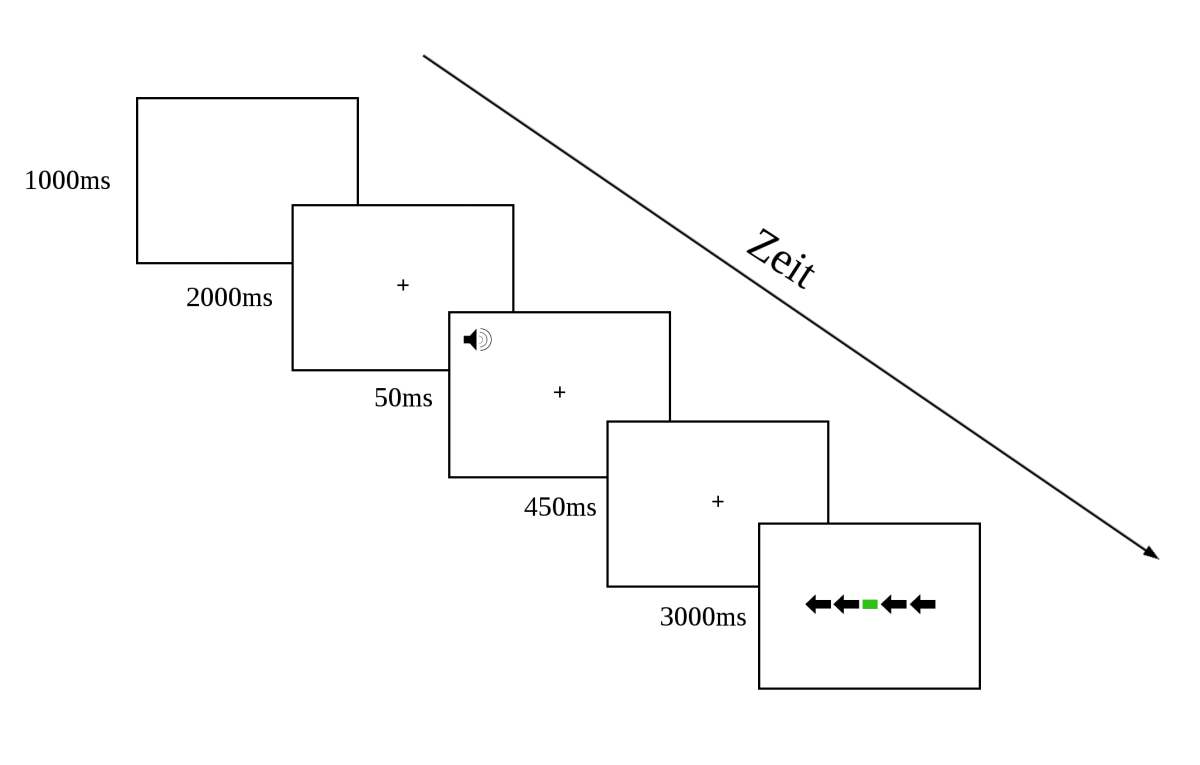
\includegraphics[width=\textwidth]{grafiken/Ablauf.png}
	\caption{Beispiel eines typischen Trials mit auditivem Hinweisreiz.}
	\label{fig:ablauf}
\end{figure*}
\subsection{Versuchsdurchführung}
Zu Beginn jedes Durchgangs wurde den Versuchspersonen 2000 Milisekunden ein weißes Fixationskreuz (Luminanz: $40.1 cd/m^2$) der Größe 0.6°x0.6° auf der Mitte des schwarzen Bildschirms (Luminanz: $< 0.1cd/m^2$) präsentiert. In der Hälfte der Trials wurden den Versuchspersonen für 50ms ein auditiver Hinweisreiz in Form eines Sinustons ($2000 Hz$, ca. $70dB$) binaural über Kopfhöhrer und anschließend für 450ms wieder ein Fixationskreuz präsentiert. In der anderen Hälfte der Versuchsdurchgängen wurde den Probanden für 500ms ein Fixationskreuz und kein auditiver Hinweisreiz präsentiert.
Anschließend wurde den Versuchspersonen für 3000ms der Zielreiz in der Mitte des Bildschirms dargeboten, der entweder aus einem dunkelgrünen (Luminanz: $8.2 cd/m^2$) oder einem dunkelroten (Luminanz: $9.4 cd/m^2$) Rechteck der Größe 0.4°x0.6° bestand. Umgeben wurde der Zielreiz von vier in regelmäßigen Abständen angeordneten Pfeilen, welche entweder alle nach links oder nach rechts zeigen konnten. Die Größe der Pfeile betrug 0.4°x0.8°.\\
\begin{figure}[t]
	\centering
	 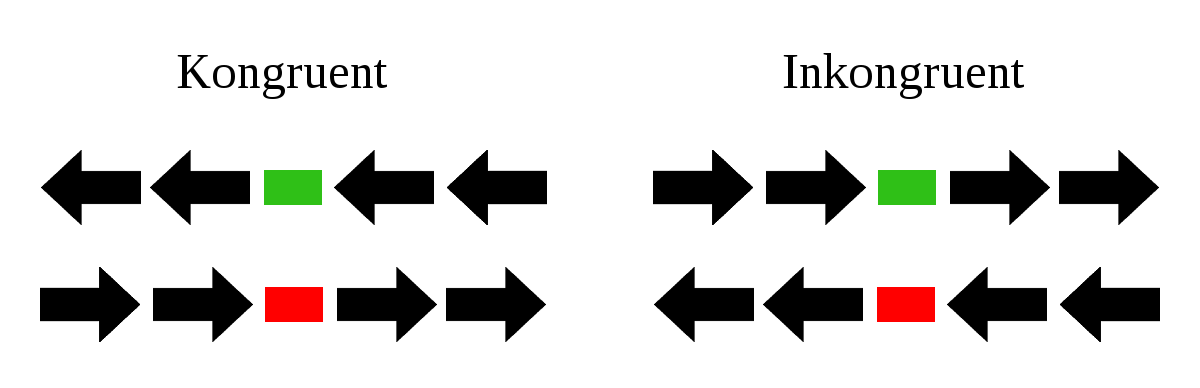
\includegraphics[width=\textwidth]{grafiken/Kongruenz.png}
		\caption{Kongruente und inkongruente Bedingung für Rechte Taste=Rot und Linke Taste=Grün}
		\label{fig:kong} 
\end{figure}
Den Versuchspersonen wurde befohlen den auditiven Reiz, sofern vorhanden, und die Flankierreize zu ignorieren und möglichst schnell auf den Zielreiz zu reagieren. Reagiert werden sollte, indem die Versuchsperson auf die der Farbe zugeordneten Taste drückt. Die Tasten wurden entweder linke Taste für Rot und rechte Taste für Grün oder umgekehrt für alle Blöcke zugeordnet und mussten mit dem Zeigerfinger der entsprechenden Hand bedient werden.\\
Die kongruente Bedingung bestand darin, dass die Richtung der Pfeile mit der Reaktion auf die Pfeile identisch war (z.B. sollte mit der rechten Hand reagiert werden und die Pfeile zeigten nach rechts).
Die inkongruente Bedingung bestand darin, dass die Richtung der Pfeile mit der Reaktion auf die Pfeile nicht identisch war (z.B. sollte mit der rechten Hand reagiert werden und die Pfeile zeigten nach links).\\
Zu Beginn der Studie erhielten die Versuchspersonen eine schriftliche Instruktion und mussten ihre demografischen Daten (Name, Alter, Sehhilfe) angeben. Nach dem sie die Instruktionen gelesen hatten, hatten sie die Möglichkeit, Fragen zu stellen. Anschließend folgte ein Übungsblock mit 24 Durchgängen, nachdem sie nochmals die Möglichkeit hatten Fragen zu stellen. Während des Übungsblocks erhielten die Versuchspersonen ein kurzes Feedback, ob ihre Eingabe korrekt war.\\
Die darauffolgenden 9 Experimentalblöcke bestanden jeweils aus 48 Versuchsdurchgängen. In jedem Block wurde jede der 12 Bedingungen 4 mal in zufälliger Reihenfolge präsentiert. Nach jedem Experimentalblock erhielten die Versuchspersonen ein Feedback über die Anzahl der korrekten Eingaben während des Blocks.\\
Am Ende des Experiments wurden die Probanden über die Hintergründe des Experiments aufgeklärt.

\subsection{Versuchsdesign}
Der Untersuchung liegt ein 2x2x3-faktorielles Design mit Messwiederholung zugrunde. Wir manipulierten dabei die Faktoren Ton (mit oder ohne Ton), Kongruenz zwischen den Zielreizen (kongruent oder inkongruent) und die Distanz der Flankierreize (0.05°, 0.1°, 0.2°).\\
Zusätzlich wurde die Tastenzuordnung, also Reaktionsrichtung auf die Farben, in beiden Möglichkeiten (rechts rot, links grün und rechts grün, links rot) zufällig den Versuchspersonen zugeordnet.\\
Als abhängige Variable wurde die Reaktionszeit und die Fehlerrate erfasst.

	
	\section{Ergebnisse}
	Reaktionszeiten, die kleiner waren als 200 ms oder größer waren als 1.000 ms, wurden von der Analyse ausgelassen (dies betraf weniger als 3\% der Trials). Der Anteil der korrekten Trials betrug 97\%. Die Reaktionszeiten für korrekte Versuchsdurchgänge in den einzelnen Versuchsbedingungen wurde analysiert mit den unabhängigen Faktoren Ton (mit Ton, ohne Ton), Kongruenz (kongruente Bedingung, inkongruente Bedingung) und Distanz (0.05°, 0.1°, 0.2°).\\
Die Analyse zeigte Haupteffekte für Kongruenz und Ton, $F(1,22)=25.20$, $p<.001$ und $F(1,22)=29.17$, $p<.001$. Die Interaktion zwischen Ton und Kongruenz war nicht signifikant, $F(1,22)=1.57$, $p=.22$. Die Interaktionen zwischen der Distanz und der Kongruenz und zwischen der Distanz und Ton waren beide nicht signifikant, $F(2,44)=0.99$, $p=.38$ und $F(2,44)=0.43$, $p=.65$. Die dreifache Interaktion zwischen Kongruenz, Ton und Distanz war ebenfalls nicht signifikant, $F(2,44)=0.63$, $p=.54$.

	
	\section{Diskussion}
	Das Ziel unserer Studie war es, zu überprüfen, ob die Interaktion zwischen Aufmerksamkeitsaktivierung und bewusster Aufmerksamkeitslenkung zu einer erhöhten räumlichen Aufmerksamkeit führt. Wir erweiterten dazu das vierte Experiment der Studie von \textcite{weinbach2012relationship} und manipulierten zusätzlich die Distanz der Flankierreize.
Wir haben erwartet, dass ein Ton die Abhnahme des Kongruenzeffekts mit der Distanz reduziert. Unsere Idee war es, dass, wenn sich der räumliche Fokus durch den Warnreiz weiten sollte, die Distraktoren auch bei größeren Abständen wahrgenommen werden würden und sich der Kongruenzeffekt daher weniger stark abschwächt.\\
\begin{figure*}[t]
	\centering
  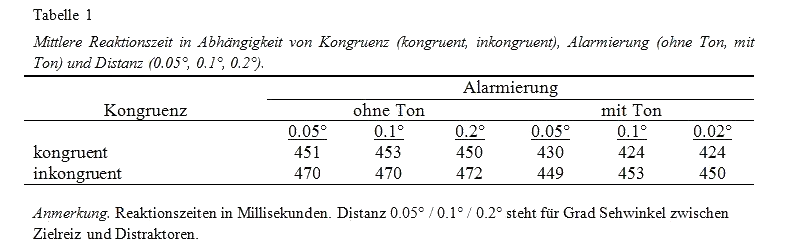
\includegraphics[width=\textwidth]{grafiken/Table-Kong_RT.png}
\end{figure*}
Diese Interaktion konnten wir nicht nachweisen. Ein möglicher Grund hierfür ist, dass wir unsere Distanzunterschiede mit 0.05°, 0.1° und 0.2° zu gering gewählt haben. Frühere Studien, welche eine Interaktion zwischen Distanz und Kongruenz nahe gelegt haben, verwendeten größere Distanzen \cite{eriksen1974effects}. Auch einen Haupteffekt für Distanz, wie ihn \textcite{eriksen1974effects} gefunden haben, konnten wir nicht finden. Dies ist möglicherweise ebenfalls auf die von uns verwendeten Distanzen zurückzuführen.\\
Auch die Ergebnisse des vierten Experiments von \textcite{weinbach2012relationship} konnten wir nicht vollständig replizieren. Es zeigten sich verkürzte Reaktionszeiten in den kongruenten Bedingungen, $F(1,22)=25.20$, $p<.001$, und in den Bedingungen mit Ton, $F(1,22)=29.17$, $p<.001$, was auch in Tabelle 1 dargestellt ist. Einen signifikanten Interaktionseffekt zwischen den beiden Faktoren, in unserem Experiment $F(1,22)=1.57$, $p=.22$, konnten wir nicht replizieren.
Eine Erklärung hierfür ist vermutlich unsere nicht exakte Replikation des Experiments, da wir dieses in einigen Punkten abgeändert haben. Zum einen verwendeten wir dunklerer Farben, welche zu einem schwereren Erkennen des Zielreizes geführt haben könnten. Es wäre also anzunehmen, dass unser Experiment schwieriger gewesen sein könnte und die mittleren Reaktionszeiten unserer Probanden daher langsamer gewesen wären. Die Analyse unserer Daten zeigte jedoch, dass die Reaktionszeiten mit denen der Probanden von \textcite{weinbach2012relationship} vergleichbar sind, wie in Abbildung~\ref{fig:vergleich} zu sehen ist.\\
Dies kann aber auch damit zusammenhängen, dass wir im Gegensatz zu \textcite{weinbach2012relationship} keine neutrale Bedingung in unserem Versuchsdesign hatten. Daraus folgt, dass die Trials mit inkongruenter Bedingung im Verhältnis zur Gesamtheit weniger werden und man daher seltener einen inkongruenten Trial erwartet. Es wäre daher anzunehmen, dass der Kongruenzeffekt in Experimenten mit neutraler Bedingung stärker ist.\\
Des Weiteren haben wir im Gegensatz zu \textcite{weinbach2012relationship} unsere Probanden in zwei Gruppen unterteilt, um beide Farb-Hand-Zuweisungen testen zu können. Jedoch zeigten auch die Einzelauswertungen nach Farb-Hand-Zuweisung keine nennenswerten Unterschiede zur Gesamtauswertung.\\
\begin{figure}[t]
	\centering
		\begin{subfigure}[b]{0.49\textwidth}
	       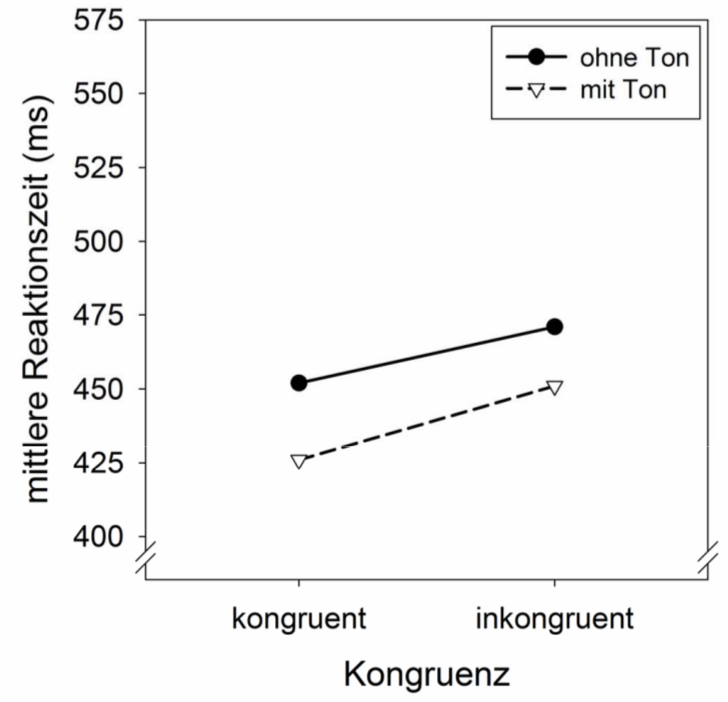
\includegraphics[width=\textwidth]{grafiken/Vergleich-unser.png}
	       \caption{Unser Experiment}
	       \label{fig:exp1}
	    \end{subfigure}%
	       ~
	    \begin{subfigure}[b]{0.49\textwidth}
	       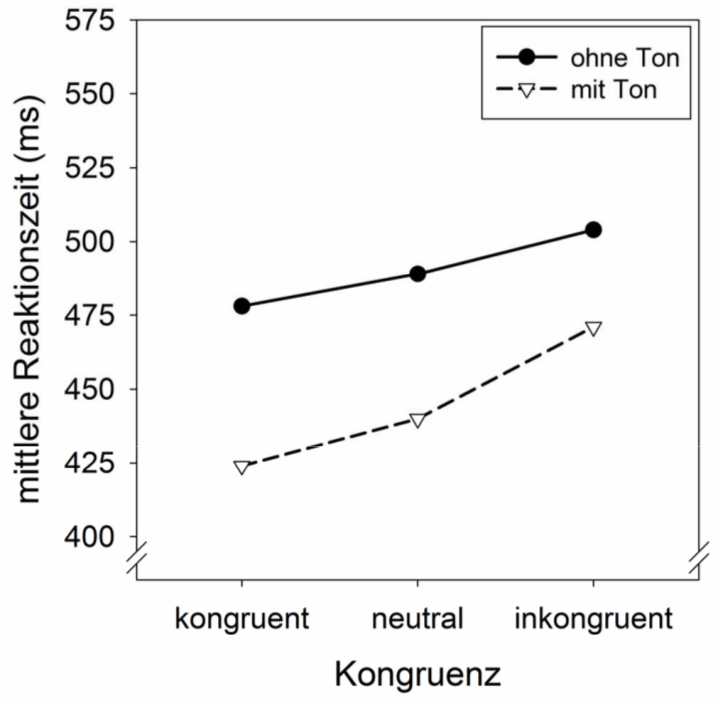
\includegraphics[width=\textwidth]{grafiken/Vergleich-henik.png}
	       \caption{Henik und Weinbach (2012)}
	       \label{fig:exp2}
	    \end{subfigure}
		\caption{Mittlere Reaktionszeiten im Vergleich}
		\label{fig:vergleich} 
\end{figure}
Evidenz für unser Hypothese konnten wir aus den zuvor genannten Gründen nicht nachweisen. Die Probleme, welche unserem Versuchsaufbau zu Grunde liegen, lassen sich jedoch leicht vermeiden. In einem möglichen Nachfolgeexperiment sollten die Distanzunterschiede vergrößert werden. Eine mögliche Größe der Distanzunterschiede könnten die bereits von \textcite{eriksen1974effects} erfolgreich verwendeten Abstände von 0.06°, 0.5° und 1° sein.\\
Da wir auch den Interaktionseffekt aus dem Experiment von \textcite{weinbach2012relationship} nicht replizieren konnten, sollte man, bevor man weitere Untersuchungen in Betracht zieht, ihr Experiment vollständig replizieren. Hierbei könnte man auch testen, wie sich die Interaktion bei anderen Distraktoren verhält. Als mögliche andere Distraktorreize könnte man die Buchstaben, welche \textcite{eriksen1974effects} in ihrer Untersuchung verwendeten, benutzen. Anschließend wäre eine Wiederholung unseres Experiments mit vergrößerten Distanzen und einer neutralen Bedingung möglich, um die Fehler aus unserer Untersuchung zu vermeiden.\\
Die Mechanismen, die unserer Aufmerksamkeitaktivierung zu Grunde liegen, benötigen weitere Untersuchungen, um unser Wissen über eine unserer zentralen kognitiven Fähigkeiten, der Aufmerksamkeit, zu erweitern. Obwohl wir mit unserer Studie nur wenig neue Erkenntnisse zu diesem spannenden Thema sammeln konnten, liefert unsere Untersuchung Erkenntnisse, die helfen können, die von uns gemachten Fehler in zukünftigen Studien zu vermeiden. 

	
	\printbibliography

	\newpage
	\section*{Erklärung}
	Hiermit erkläre ich, dass ich diesen Abschlussbericht selbständig verfasst habe, keine anderen als die angegebenen Hilfsmittel und Quellen benutzt habe und alle wörtlich oder sinngemäß aus anderen Werken übernommenen Aussagen als solche gekennzeichnet habe.\\
\\
\\
Tübingen, den \today
\\
\\
\\
------------------------------------\\
\textsc{\large \vorname \space \name}
\end{document}
